\documentclass[12pt]{article}
\setlength{\oddsidemargin}{0in}
\setlength{\evensidemargin}{0in}
\setlength{\textwidth}{6.5in}
\setlength{\parindent}{0in}
\setlength{\parskip}{\baselineskip}
\usepackage[edges]{forest}
\usepackage{amsmath,amsfonts,amssymb}
\usepackage{graphicx}
\usepackage{fancyhdr}
\pagestyle{fancy}



\begin{document}

\lhead{{\bf CSCI 3104: Algorithms \\ Problem Set 4} }
\rhead{{\bf Rhett\ Hanscom\\ Summer 2019, CU-Boulder}}
\renewcommand{\headrulewidth}{0.4pt}

% 15+45+20+20=100 points possible

\vspace{-3mm}
\begin{enumerate}

	% -- MEDIUM PROBLEM
	\item (15 points) Shadow is writing a secret message to Harry and wants to prevent it from being understood by Thormund. He decides to use Huffman encoding to encode the message. Magically, the symbol frequencies of the message are given by the Lucas numbers, a famous sequence of integers discovered by the same person who discovered the Fibonacci numbers. The nth Lucas number is defined as $L_n = L_{n-1} + L_{n-2}$ for $n > 1$ with base cases $L_0$ = 2 and $L_1$ = 1.
	\begin{enumerate}
	\item \label{q:huff:a} For an alphabet of $\Sigma=\{a,b,c,d,e,f,g,h\}$ with frequencies given by the first $|\Sigma|$ Lucas numbers, give an optimal Huffman code and the corresponding encoding tree for Shadow to use.
	
	\item Generalize your answer to (\ref{q:huff:a}) and give the structure of an optimal code when the frequencies are the first $n$ Lucas numbers.
	
	\end{enumerate}

\pagebreak
\textbf{Solution to Problem 1:}

\begin{enumerate}
    \item 


    \begin{forest}
    for tree={
        grow=south,
        circle, draw, minimum size=3ex, inner sep=1pt,
        s sep=7mm
            }
    % [51
    %     [12
    %         [1]
    %         [43
    %             [36]
    %         ]
    %     ]
    %     [87
    %         [52
    %             [83]
    %         ]
    %     ]
    % ]
    
    [75 
        [H]
        [46
            [G]
            [28
                [F]
                [17
                    [E]
                    [10
                        [D]
                        [6
                            [C]
                            [3
                                [B]
                                [A]
                            ]
                        ]
                    ]
                ]
            ]
        ]
    ]
    \end{forest}
    
    \begin{left}
    \begin{tabular}{ |c|c| } 
    \hline
    Letter & Frequency \\
     \hline
     A & 2 \\
     B & 1 \\
     C & 3 \\
     D & 4 \\
     E & 7 \\
     F & 11 \\
     G & 18 \\
     H & 29 \\
     
     \hline
    \end{tabular}
    \end{left}
    
    \begin{right}
    \begin{tabular}{ |c|c| } 
    \hline
    Letter & Huffman Code \\
     \hline
     A & 1111111 \\
     B & 1111110 \\
     C & 111110 \\
     D & 11110 \\
     E & 1110 \\
     F & 110 \\
     G & 10 \\
     H & 0 \\
     
     \hline
    \end{tabular}
    \end{right}
    
    \item
    When constructing a tree based on the greedy Huffman Algorithm, we first use the two objects with the lowest frequencies and and the first sub tree with these nodes. The sum of their frequencies becomes their parent. Next, we obtain the next node remaining with the lowest frequency and this become the second child node of the newly created node representing the fist sum node. The sum of this node and the previously used node then becomes the highest parent node in this tree. As the Lucas numbers only sum the previous two numbers and our tree will create parent nodes summing all of their children, we will never have a case where the lowest frequency letter cannot be placed as a sibling to the most recently generated parent node.
    
    A patter for this process quickly emerges wherein for \textit{n} letters have the pattern:
    $Letter_{0}$ = 11111...0 where 1 appears \textit{n}-1 times \\
    $Letter_{1}$ = 1111....0 where 1 appears \textit{n}-2 times \\
    $Letter_{2}$ = 111.....0 where 1 appears \textit{n}-3 times \\
     . \\
     . \\
     . \\
    $Letter_{n}$ = 0 where 1 appears \textit{n}-n (zero) times \\

\end{enumerate}

	% HARD PROBLEM
	\item (45 points) A good hash function $h(x)$ behaves in practice very close to the uniform hashing assumption analyzed in class, but is a deterministic function. That is, $h(x)=k$ each time $x$ is used as an argument to $h()$. Designing good hash functions is hard, and a bad hash function can cause a hash table to quickly exit the sparse loading regime by overloading some buckets and under loading others. Good hash functions often rely on beautiful and complicated insights from number theory, and have deep connections to pseudorandom number generators and cryptographic functions. In practice, most hash functions are moderate to poor approximations of uniform hashing.
	
	\smallskip Consider the following hash function. Let $U$ be the universe of strings composed of the characters from the alphabet $\Sigma=[${\tt A}$,\dots,${\tt Z}$]$, and let the function $f(x_{i})$ return the index of a letter $x_{i}\in \Sigma$, e.g., $f(${\tt A}$)=1$ and $f(${\tt Z}$)=26$. Finally, for an $m$-character string $x\in \Sigma^{m}$, define $h(x) = \left(\left[\sum_{i=1}^{m}f(x_{i})\right]\!\! \mod \ell\right)$, where $\ell$ is the number of buckets in the hash table. That is, our hash function sums up the index values of the characters of a string $x$ and maps that value onto one of the $\ell$ buckets.
	
	\begin{enumerate}
    	\item The following list contains US Census derived last names: \\
    	{\tt http://www2.census.gov/topics/genealogy/1990surnames/dist.all.last} \\
    	Using these names as input strings, first choose a uniformly random 50\% of these name strings and then hash them using $h(x)$.
    	
    	Produce a histogram showing the corresponding distribution of hash locations when $\ell=200$. Label the axes of your figure. Briefly describe what the figure shows about $h(x)$, and justify your results in terms of the behavior of $h(x)$. Do not forget to append your code.
    	 
    	{\footnotesize Hint: the raw file includes information other than name strings, which will need to be removed; and, think about how you can count hash locations without building or using a real hash table.}
    	
    	\item Enumerate at least 4 reasons why $h(x)$ is a bad hash function relative to the ideal behavior of uniform hashing.
    	
    	\item Produce a plot showing (i) the length of the longest chain (were we to use chaining for resolving collisions under $h(x)$) as a function of the number $n$ of these strings that we hash into a table with $\ell=200$ buckets, (ii) the exact upper bound on the depth of a red-black tree with $n$ items stored, and (iii) the length of the longest chain were we to use a uniform hash instead of $h(x)$. Include a guide of $c\,n$
    	
    	Then, comment (i) on how much shorter the longest chain would be under a uniform hash than under $h(x)$, and (ii) on the value of $n$ at which the red-black tree becomes a more efficient data structure than $h(x)$ and separately a uniform hash.
	\end{enumerate}

\pagebreak
\textbf{Solution to Problem 2:}

\begin{enumerate}
\item
\begin{figure}
    \centering
    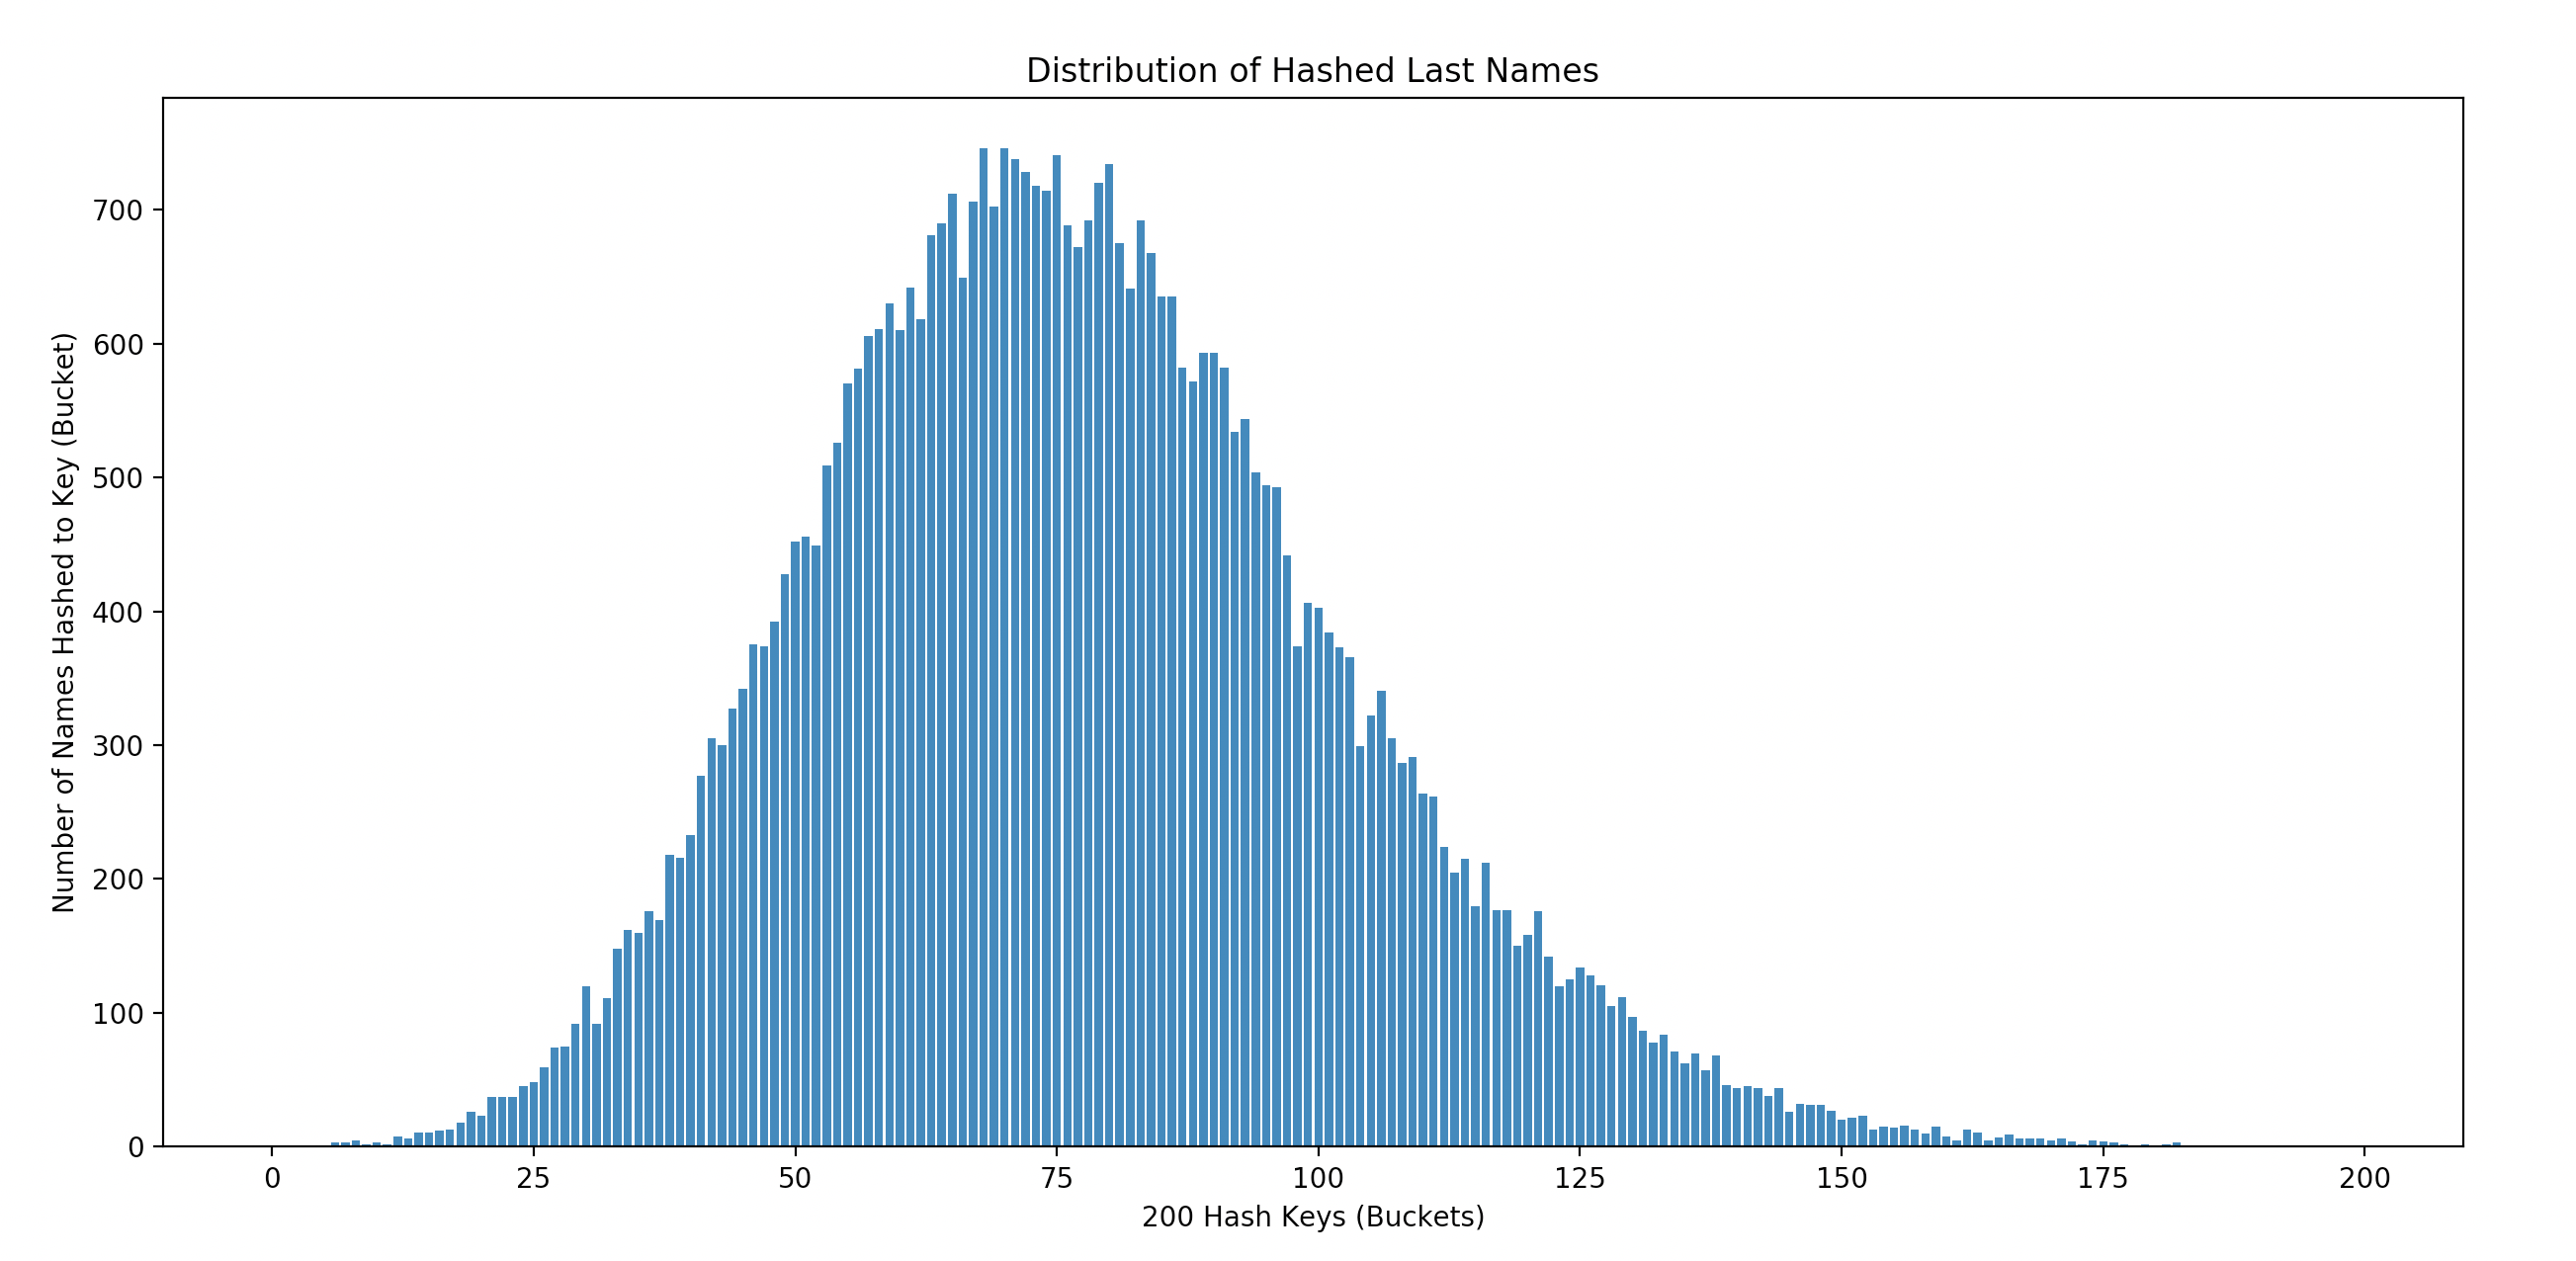
\includegraphics[width=0.8\linewidth]{histogram_PS4.jpeg}
    \caption{The code for this histogram is included in the attached .zip file in the PS4\_2A\_Histogram.py}
    \end{figure}
Histogram showing the distribution of keys when hashing by last name with $\Sigma$ letter value and then mod'ed by the bucket size (pictured above).
\item
4 reasons this hash function is not optimal:
\begin{enumerate}
\item No value is placed on the placement of the letters with this hash function. Permutations are not accounted for, i.e., the string "ABC" would have the same value as "CAB".
\item Last names tend to have a similar number of letters, this further reduces the spread of hash values.
\item Last names tend to have similar letters in addition to similar lengths. This leads to even more lumping around mid-ling buckets. For example, nearly every last name will have multiple vowels whereas very few last names will feature the letters z of x proportionally.
\item The mod feature used simply in conjunction with the sum of the letter values makes it quite hard to achieve a very low score. Aside from having the last name 'A', to achieve a hash of one or a similarly small value a last name would need to contain 15 or more letters if we assume a mean letter value of 13.
\end{enumerate}
\newpage
\item
\begin{figure}
    \centering
    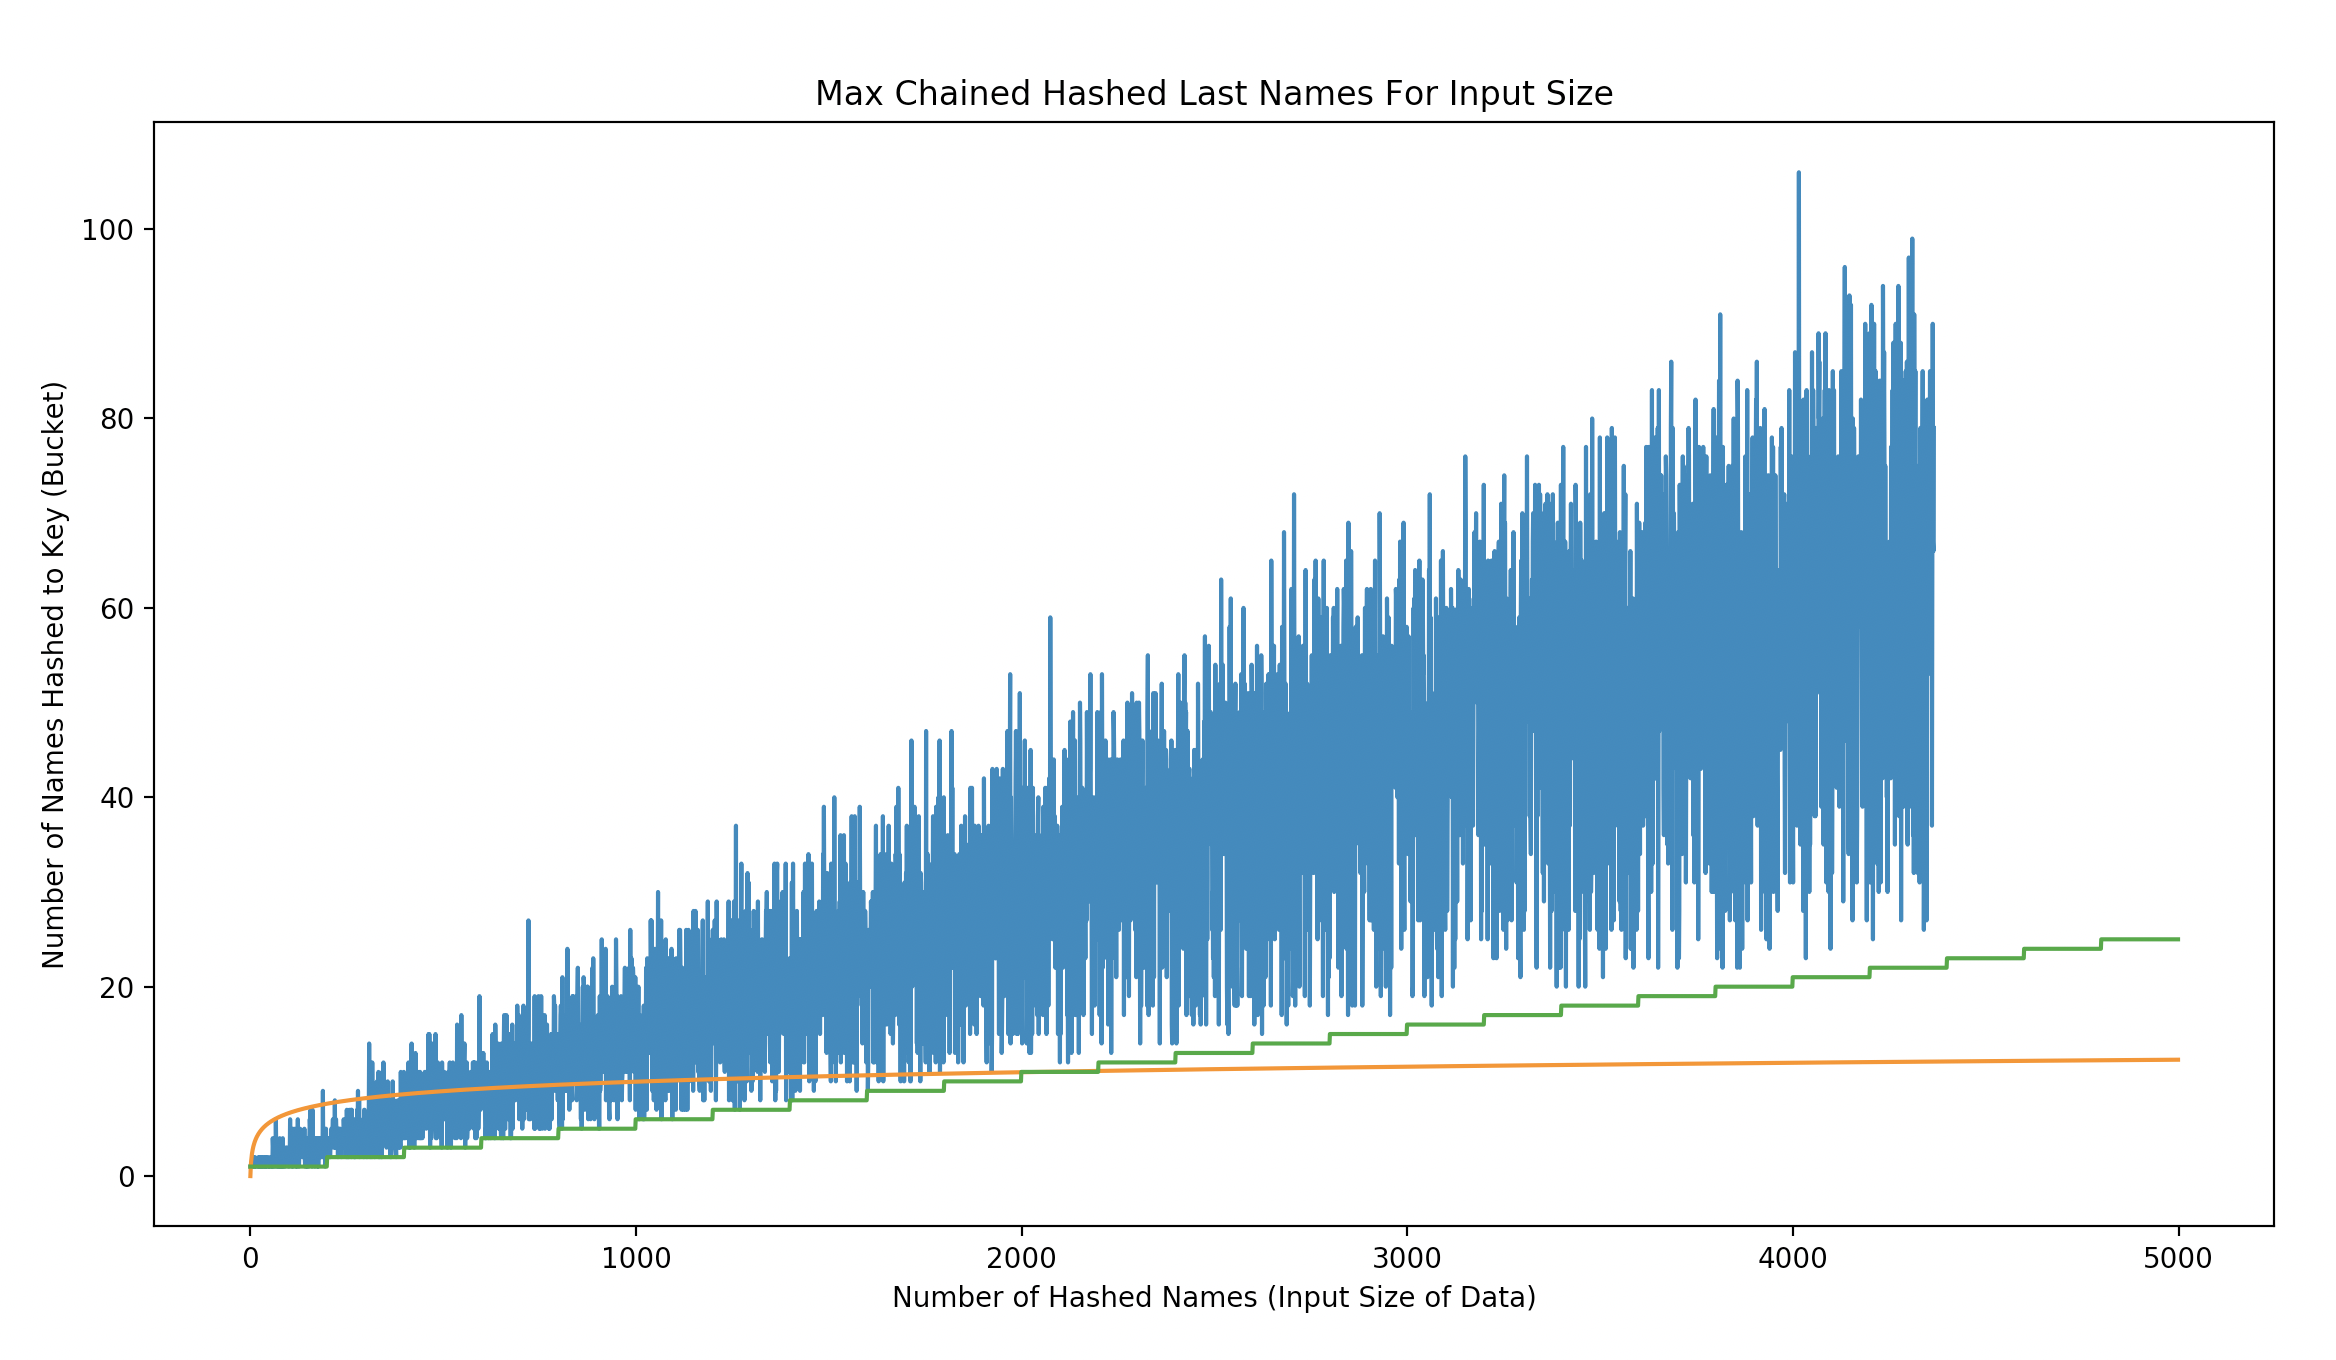
\includegraphics[width=0.9\linewidth]{plot.jpeg}
    \caption{In the above figure, the blue represents the maxim values for our hash function, the orange is the $log_{2}(x)$ and the green is the uniform hash function. The code for this plot is included in the .zip file within the program named PS4\_2C\_Plot.py}
    \end{figure}

In the above plot, the exact upper bound on the depth of a red-black tree with \textit{n} items is represented by the function $log_{2}(x)$, and the length of uniform hashing is represented by a the green function, which takes a step up for each time the data size increases by 200 (the number of buckets).

\begin{enumerate}
    \item When using our hash function, \textit{h(x)}, there tend to be four times as many values hashed into the most used bucket than when using a uniform hashing function.
    \item When using a red and black tree, value of \textit{n} at which the red-black tree becomes a consistently more efficient data structure than h(x) is around a data input size of 300. The uniform hashing function performs as well as or better than \textit{h(x)} from the very beginning. The uniform hashing function becomes obviously more efficient as early as \textit{n} = 25.
\end{enumerate}
\end{enumerate}

\newpage
	% MEDIUM PROBLEM
	\item (20 points) Grog is struggling with the problem of making change for $n$ cents using the smallest number of coins for his purchase of a new great sword. Grog has coin values of $v_{1}<v_{2}<\dots<v_{r}$ for $r$ coin types, where each coin's value $v_{i}$ is a positive integer. His goal is to obtain a set of counts $\{d_{i}\}$, one for each coin type, such that $\sum_{i=1}^{r}d_{i}=k$ and where $k$ is minimized.
	\begin{enumerate}
	\item A greedy algorithm for making change is the \textbf{cashier's algorithm}, which all young wizards learn. Harry writes the following pseudocode on the whiteboard to illustrate it, where $n$ is the amount of money to make change for and $v$ is a vector of the coin denominations:
	%
	\begin{small}
	\begin{verbatim}
	wizardChange(n,v,r) :
	   d[1 .. r] = 0       // initial histogram of coin types in solution
	   while n > 0 {
	      k = 1
	      while ( k < r and v[k] > n ) { k++ }
	      if k==r { return 'no solution' }
	      else { n = n - v[k] }
	   }
	   return d
	\end{verbatim}
	\end{small}
	Thormund snorts and says Harry's code has bugs. Identify the bugs and explain why each would cause the algorithm to fail.
	
	\item Sometimes the dwarves at Rocky Mountain Bank run out of coins,%
	%
	\footnote{It's a little known secret, but dwarven pets like to \textit{eat} the coins. It isn't pretty for the coins, in the end.}
	%
	and make change using whatever is left on hand. Identify a set of U.S. coin denominations for which the greedy algorithm does not yield an optimal solution. Justify your answer in terms of optimal substructure and the greedy-choice property. (The set should include a penny so that there is a solution for every value of $n$.)


%	1. Greedy-choice property: A global optimum can be arrived at by selecting a local optimum.
%	2. Optimal substructure: An optimal solution to the problem contains an optimal solution to subproblems.
	
	\item On the advice of wizards specializing in electricity, Rocky Mountain Bank has announced that they will be changing all  coin denominations into a new set of coins denominated in powers of $c$, i.e., denominations of $c^{0}, c^{1}, \dots , c^{\ell}$ for some integers $c>1$ and $\ell\geq 1$.  (This will be done by a spell that will magically transmute old coins into new coins, before your very eyes.) Prove that the cashier's algorithm will always yield an optimal solution in this case.
	
	Hint: first consider the special case of $c=2$.

	\end{enumerate}
 
\pagebreak
\textbf{Solution to Problem 3:}
\begin{enumerate}
\item
\begin{verbatim}
wizardChange(n, v, r):
    d[1 .. r] = 0
    while n > 0 {
        k = 1
        while ( k <= r and v[k] > n ) {k++}
        if k > r {return 'no solution'}
        else { n = n - v[k]
            d[k]++
            }
        }
    return d
\end{verbatim}

\item
\$ Dollar denominations = [.1, .10, .25], Value to achieve: \$.30 \newline
Our algorithm chooses [.25, .1, .1, .1, .1, .1] equalling six coins used to create this value. Here we see that when looking to make change for the value of \$.30, the algorithm will first choose the use a \$.25 coin and then five pennies to achieve the correct total of \$.30. However, the more optimal solution to this problem would have \$.30 achieved by using three \$.10 coins, therein using half the number of coins our algorithm recommends. 

\item Consider our base case of $\textit{l}$ = 1, we would have coins of only value 1 and value C. As many C coins as could be used would be used to achieve any value and then only coins worth 1 would remain to attain the desired value.

Now, let us looks toward larger coins. Consider coins of $C^{k}$ and $C^{k-1}$ for \textit{k} \textless \textit{l}. We could only ever use C-1 $C^{k-1}$ coins before we would have been forced to select an additionally $C^{k}$ coin in the previous selection process. If this logic is applied to each value of \textit{k} from \textit{l} to 0, there would be no opportunity to select a coin which would lead to a non-optimal solution.
\end{enumerate}

    \item (20 points) We saw in the previous problem that the cashier's (greedy) algorithm for making change doesn't handle arbitrary denominations optimally. In this problem you'll develop a dynamic programming solution which does, but with a slight twist. Suppose we have at our disposal an arbitrary number of \emph{cursed} coins of each denomination $d_1, d_2, \dotsc, d_k$, with $d_1 < d_2 < \dotsc < d_k$, and we need to provide $n$ cents in change. We will always have $d_1=1$, so that we are assured we can make change for any value of $n$. The curse on the coins is that in any one exchange between people, with the exception of $i=2$, if coins of denomination $d_i$ are used, then coins of denomination $d_{i-1}$ \emph{cannot} be used. Our goal is to make change using the minimal number of these cursed coins (in a single exchange, i.e., the curse applies).

    \begin{enumerate}
    	\item For $i \in \{1,\dotsc,k\}$, $n \in \mathbb{N}$, and $b \in \{0,1\}$, let $C(i,n,b)$ denote the number of cursed coins needed to make $n$ cents in change using only the first $i$ denominations $d_1, d_2, \dotsc, d_i$, where $d_{i-1}$ is allowed to be used if and only if $i \leq 2$ or $b=0$. That is, $b$ is a Boolean ``flag'' variable indicating whether we are excluding denomination $d_{i-1}$ or not ($b=1$ means exclude it). 	
    	Write down a recurrence relation for $C$ and prove it is correct. Be sure to include the base case.
    	\item Based on your recurrence relation, describe the order in which a dynamic programming table for $C(i,n,b)$ should be filled in.
    	
    	\item Based on your description in part (b), write down pseudocode for a dynamic programming solution to this problem, and give a $\Theta$ bound on its running time (remember, this requires proving both an upper \emph{and} a lower bound).
    \end{enumerate}
\newpage

\pagebreak
\textbf{Solution to Problem 4:}

\begin{enumerate}
    \item 
    $
    C(i, n, b) =
        \begin{cases}
            b = 0
            \begin{cases}
                    $if $ n >= di 
                        \begin{cases}
                              $Min $(C(i-1, n-di, 1), C(i-1, n, 0))\\
                        \end{cases}\\
                    $else  $   C(i-1, n, 0)\\
                    \end{cases}\\
            b = 1 \begin{cases}
                        C(i-1, n, 0)\\
                        \end{cases}
            \\n = 1 \begin{cases} return 1 \end{cases}\\
        \end{cases}
    $
    
    \textbf{Proving optimal substructure}:
    Given am amount, n, i denominations of coins, and b, a bool indicating if we are allow to use this coin type C(i, n, b) returns the optimal solution (minimum number of coins to achieve this amount).
    
    \textbf{Case 1}: b == 1, we cannot use this coin, therefore we decrease i by 1 to look at the next coin type we are able to use. Additionally, we ensure that b is changed to 0 to ensure it is indicated we are able to use the next coin type considered.
    
    Suppose there is a C'(i-1, n, 0) that gives more optimal substructure (C'(i-1, n, 0) \textless C(i-1, n, 0)). If we are unable to use this coin type, we add 0 (number of coins used) + C'(i-1, n, 0), which will give us a new optimal substructure. 0 + C'(i-1, n, 0) \textless C(i-1, n, 0), a contradiction.
    
    \textbf{Case 2}: b == 0, we can use this coin type, here we have two more cases and we chose the case which produces the smallest number of coins:
    
    \textbf{Case 2A}: n is less than the value of i, we cannot use this coin, so we add 0 + C(i-1, n, 0). We have proven this is the most optimal substructure when no coin is used in Case 1.
        
    \textbf{Case 2B}: n is greater than the value of i, here we can either use the coin or go down to another, smaller coin type. 
    
    If do not take the coin, we add 0 + C(i-1, n, 0). We have proven this is the most optimal substructure when no coin is used in Case 1.
    
    If we do take the coin, we add 1 + C(i-1, n-value(i), 1). Suppose there is another C function such that C'(i-1, n-value(i), 1) \textless C(i-1, n-value(i), 1), indicating that a more optimal substructure is available. If we take the coin we add 1 + C'(i-1, n-value(i), 1), which will give us a new optimal substructure for 1 + C'(i-1, n-value(i), 1) \textless C(i-1, n-value(i), 1), a contradiction.
    
    
    
    
    Now, to prove the entire recurrence relation produces optimal results:
    
    
    \textbf{Theorem 1} - Given an amount, n, i denominations of coins, and b, a bool indicating if we are allow to use this coin type C(i, n, b) returns the optimal solution (minimum number of coins to achieve this amount). There will always be a coin worth a value of 1 available.
    
    
    \textbf{Inductive Hypothesis} - Assume that Theorem 1 holds for values of x \textless n or for coin types i \textless k.
    
    
    \textbf{Base Case} - (x = 1) If the amount we are looking to make change for is 1, we give them a single coin worth 1, it is the only choice and the problem states this coin is always available. 
    
    
    \textbf{Inductive Step} - 
    For an arbitrary x and i we have two cases to consider:
    X is greater than the value of i, in which case we can either use the coin or chose not to. Here we chose the sequence which produces the minimum number of coins either 1 + C(i-1, n-value(i), b) or 0 + C(i-1, n, b). In each case, either n is greater than n-value(i) or i is greater than i - 1 and we are able to apply our Inductive hypothesis.
     
        
    X is less than i, here we cannot use it. Therefore we must look at the i-1 coin. This is the only option and is trivially correct.
        
    
    Thus this relation has been proven optimal. 
    
    
    \item
    Assuming the array is built with decreasing n values along the x axis and increasing values of coins along the y axis, this matrix will be filled in beginning with the topmost left indexes and then gradually grow downward and rightward as we fill in these indexes with their optimal solutions. This is the point of dynamic programming, we rely on previously generated answers to assist with our solution moving forward as opposed to generating the same answer to the same equation multiple times. 
    
    \item
    
    \begin{verbatim}
def C(i, n, b):

	matrix = []
	matrix_b = []
	for coin in range(0, i):
	    matrix[0, coin] = 0 #top row all zeros as the amount is zero
	for x = 0 to i:
	    for y = 0 to n:
	        if x > 0 & y > 0:
	            if y >= value(x) and matrix_b[x-1, n] != 1:
	                 matrix[x,y] = Min(matrix[x-1, y-value(x)], matrix[x-1, y])
            elif y >= value(x) and matrix_b[x-1, n] == 1:
                matrix[x,y] = matrix[x-1, y])
	return matrix[i, n]
    \end{verbatim}
    
    The two for-loop in this dynamic programming algorithm results in a \theta (n^{2}).
\end{enumerate}

\end{enumerate}



\end{document}

